\documentclass[main.tex]{subfiles}

\begin{document}
\section{Overview}
A large number of charged cosmic ray events are included among the triggering events despite the three-level trigger. Most current generation experiments use analysis techniques based on \cite{Hillas:1985}, using the second moments of the distribution of pixel signal amplitudes, which for VERITAS, yield an angular resolution of $\sim <0.1^\circ$ at 1 TeV. However, significantly more information can be extracted from the recorded data using a template library containing expected shower images for a given set of shower parameters. This template library can then be compared to the recorded images for any given event and the best-fit shower parameters can be determined resulting in improved resolution in direction and energy reconstruction. This section provides a brief overview of the Monte-Carlo simulations used to generate these templates for VERITAS.

\section{Shower Generation}
This section describes the prediction of the expected Cherenkov light distribution in the camera focal plane for a given set of primary particle parameters. The production of mean shower images is divided into two steps: the generation of large Monte Carlo datasets of air showers and the simulation of the detector response. The electromagnetic air showers in the atmosphere are simulated with the CORSIKA (COsmic Ray SImulations for KAscade) program and simulations are performed over a range of parameters like energy, zenith angle and impact distance. 

In the simulation, which contains the shower generation from \ref{Gamma-ray-EAS}, when a charged particle exceeds $v>c/n$, Cherenkov photons are generated. The number of photons emitted is calculated for a given extent of the path and the propagation directions are randomly selected from the surface of a Cherenkov cone (i.e. $\theta_c = \cos^{-1}\beta/n$). Each photon is then tracked through the atmosphere until it reaches the altitude of the observatory. CORSIKA does not track whether the photon hits a telescope reflector, but instead defines a volume around each telescope in order to filter photons to store. Photons whose trajectory does not intersect this volume are not stored.

With the camera pointing at the shower source, each of the telescope cameras lies on a plane perpendicular to the shower axis, making the shower projection plane and the camera planes parallel. The CORSIKA simulation output contains the photon distribution at the telescope altitude, and the arrival direction of each photon. For each event, the Cherenkov photons falling onto the mirror elements are tracked by their arrival times, initial direction, and wavelength. The detector response is modeled using the atmospheric density profile, optical absorption and some of the detector characteristics such as its light-collecting area, and phototube quantum efficiency. It also accounts for the physical structure of the telescopes such as occultation by the quadripod arms and the camera box. The images are produced for the VERITAS telescopes which use a Davies-Cotton design and cameras with 499 pixels, each pixel having a field of view (FOV) of 0.15$^\circ$ in diameter.

The shower images are generated for a range of first-interaction depths, energies, wobble offsets and impact distances. A multidimensional interpolation algorithm is used to interpolate between the templates, allowing production of an image template for any shower parameters within the parameter ranges. An additional parameter included here is the effect of the geomagnetic field on the electromagnetic showers \cite{Vincent:2015bnj}.
% 3. Likelihood Reconstruction & Performance
Once the full set of templates has been created, they can be compared with the observed images by performing a global fit to the telescope image data using a model for the expected pixel amplitudes. Shower parameters are determined by maximizing an array likelihood function outlined in \cite{deNaurois}.

\section{The VEGAS Analysis Package}
The VERITAS observation and simulation data contain the PMT pulses, pointing direction, time and time gradient (which are extracted from the PMT pulses), and other trigger and operational conditions. To produce a sky map, these data files are piped through a series of functions to extract, among other things, energy and direction information. At VERITAS there are two standard analysis packages for this process (\vegas  and \ed), both based in ROOT/C++, with a similar set of functions. While the analysis methods in this work can be and are applied in both analysis packages, the analysis in this work was performed using the \vegas package.
\vegas consists of 6 distinct processes, initially written as 6 distinct modules, as follows:
\begin{itemize}
\item Stage 1: Calibration Calculation -- This stage calculates the hardware dependent parameters of the VERITAS data and collects relevant information at each trigger level (pixel, telescope, and array) to determine a set of calibration parameters. The following stages can then use these parameters in conjunction with the data to remove any hardware dependence.
\item Stage 2: Calibration Application -- This stage calculates calibrated charge information for PMT traces using information on pedestals, relative gains, and relative channel timing. In more recent iterations, the analysis module for stage 2 also performs the functions previously performed in stage 3. 
\item Stage 3: Image Parameterization -- This stage removes noisy pixels using stage 1 \& 2 information and calculates the image parameters (described in \ref{shower-img-params}). This stage treats each telescope independently and so image parameters are calculated for each telescope image.
\item \textbf{Stage 4: Shower Reconstruction} -- This is the most important stage for the purposes of this work. This stage performs an array-level reconstruction of the shower, using individual telescope information to calculate \textbf{shower direction}, event energy, depth of the shower maximum, and core location.
\item Stage 5: Event Selection -- This stage is designed to apply cuts to events based on the output of the previous stages to better distinguish hadronic showers from gamma-ray showers, as well as enforce any other restrictions on telescope-image or stereoscopic parameters.
\item Stage 6: Results Extraction -- This stage calculates and displays the final results of the desired analysis -- single telescope analysis, stereoscopic analysis, spectral analysis or temporal flux analysis.
\end{itemize}
The focus of this work will be on the direction reconstruction part of stage 4.

\section{Direction Reconstruction}
\begin{figure}[htbp]
  \centering
  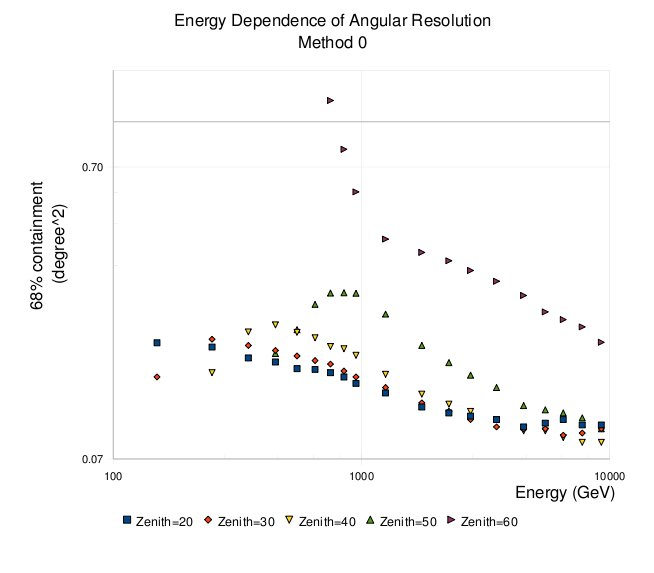
\includegraphics[width=.6\linewidth]{images/Method0_res}
  \caption[Angular resolution of Method0]{Angular resolution of Method0 direction reconstruction against energy scale and zenith angle.}
  \label{fig:disp_res}
\end{figure}
The standard method (henceforth method0) of shower direction reconstruction is based on the intersections of the major axes of Hillas ellipses. This method carries a lot of stereoscopic information and is in general very powerful. However, since for large zenith angles (LZA), one expects shower images (and therefore Hillas ellipses) in the camera plane to be close to parallel, small uncertainties in major axis determination result in large uncertainties in the fiducial location of the reconstructed gamma ray in the camera plane (the ``shower location''). As shown in Fig. \ref{fig:disp_res}, for lower energies and larger zenith angles, there is a substantial drop in angular resolution.

To compensate for this loss of predictive power, the \disp \textit{method}, calculates the \disp parameter (quasi-analytically, using lookup tables and interpolating, or using \textbf{boosted decision trees}) for each individual telescope image to determine two potential locations for the arrival direction -- along the major axis on either side of the weighted centroid of the image (see Fig. \ref{fig:hillas_ellipse}). The method then compares this pair of coordinates (one at the head, and one at the tail) for each pair of telescopes in the event reconstruction to find the pair of coordinates, one from either telescope, closest to each other (see Fig \ref{fig:head_tail} for visual explanation). The mean of this pair of coordinates is determined to be the reconstructed shower direction.
\begin{figure}[htbp]
  \centering
\subfigure[First pair of telescopes in reconstruction, with the pair of closest coordinates]{
  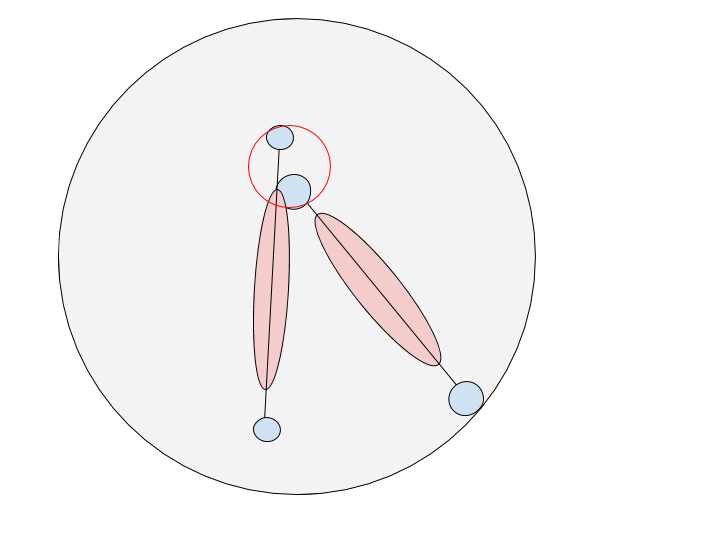
\includegraphics[width=.31\linewidth]{images/head_tail_1}
}
\subfigure[Second pair of telescopes in reconstruction, with the pair of closest coordinates]{
  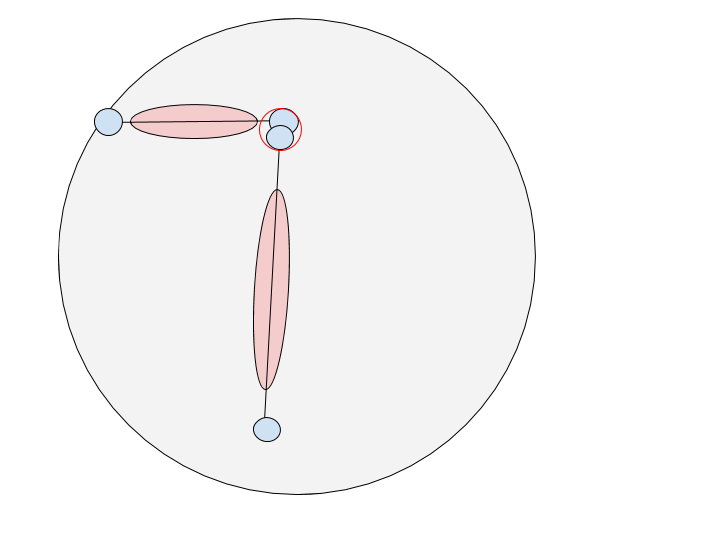
\includegraphics[width=.31\linewidth]{images/head_tail_2}
}
\subfigure[Third pair of telescopes in reconstruction, with the pair of closest coordinates]{
  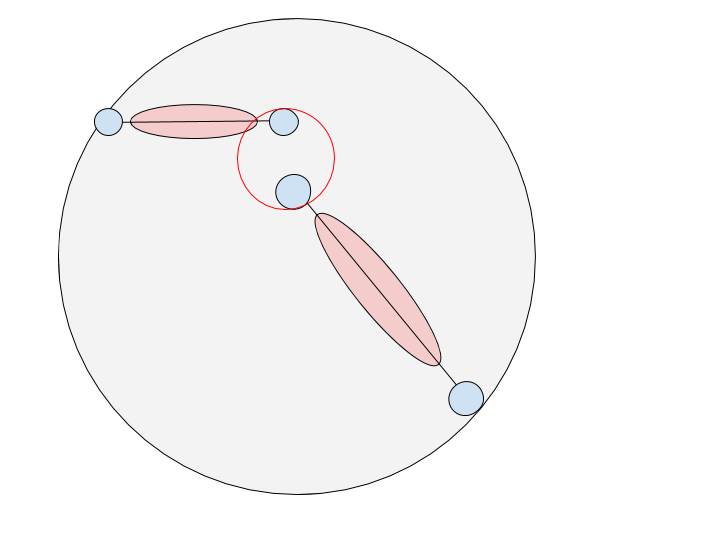
\includegraphics[width=.31\linewidth]{images/head_tail_3}
}
\subfigure[All telescopes in reconstruction, with the pair of closest coordinates from \textit{all} pairs of telescopes]{
  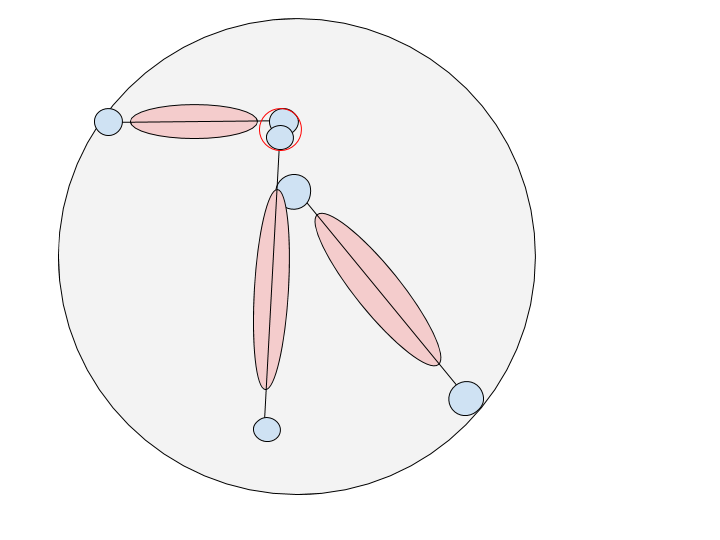
\includegraphics[width=.6\linewidth]{images/head_tail_full}
}
  \caption[Combining multiple telescopes in \disp reconstruction]{Iterating through the unique pairs of telescopes, the closest coordinate pair is chosen, and the mean of those coordinates is determined to be the direction of the initiating particle.}
  \label{fig:head_tail}
\end{figure}


\section{Boosted Decision Trees}
Decision trees use a predictive model, which maps parameters for an event to the value of the \disp parameter for the event. The predictive model may be based on Monte Carlo simulations (as in the case of this work) or analytic calculations. To avoid having multiple identical trees, a higher weight is assigned to events that are canonically hard to discriminate. This means that within the training, more time is spent on discriminating between events that are hard to distinguish and this assigning of weights to preferentially train more on specific parts of parameter space is referred to as boosting.

The implementation of the \disp method in \vegas (and \ed) uses the ROOT Toolkit for Multi-Variate Analysis (TMVA) package. The TMVA package contains implementations of several complex algorithms including neural networks, Fisher discriminants and boosted decision trees (BDTs). BDTs are especially robust for variables with non-linear correlations and have a fast application to data, relative to some of the other algorithms.

\end{document}
